\section{System Design}
\label{sec:design}

This section describes the design with UML diagrams drawn from the source code. The diagrams are generated from PlantUML files kept next to the paper. Where the code is unfinished, the figure says so.

\subsection{Use cases}

Figure~\ref{fig:usecase} shows what an observer does with the app. Dashed ovals mark use cases whose current form is in development: the revised alignment flow, the setup wizard with phone placement, and plate solving with the camera. The solver itself is written and tested, but the camera capture code is not. The other use cases are in the current build. Following guidance includes choosing a target, and a plate solve extends alignment because a solved image is meant to be applied to the alignment.

\begin{figure*}[tp]
\centering
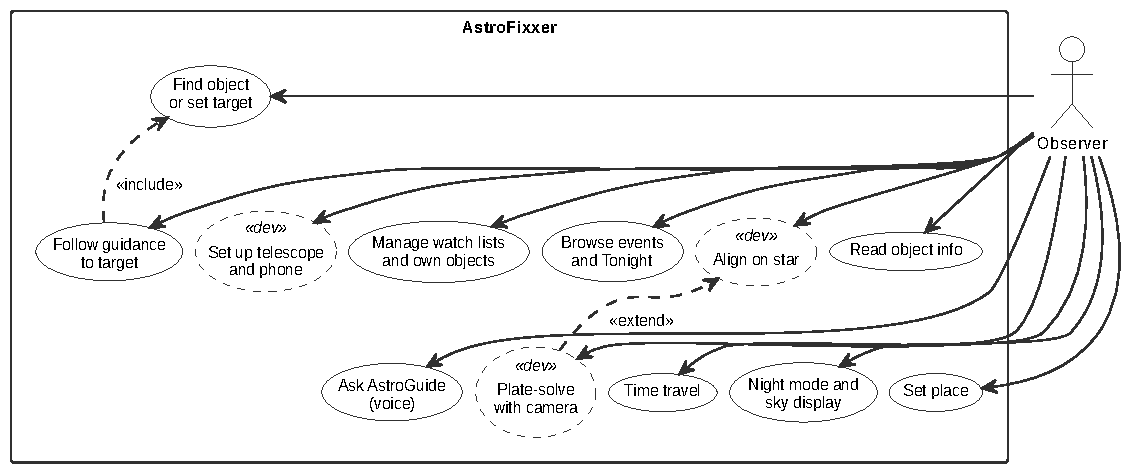
\includegraphics[width=0.9\textwidth]{figures/uml01_usecase.pdf}
\caption{Use cases of the observer. Dashed ovals are in development}
\label{fig:usecase}
\end{figure*}

\subsection{Structure}

Figure~\ref{fig:components} shows the runtime structure. \texttt{MainActivity} is the only code that touches the Android framework. It reads the rotation-vector sensor, gets a location fix, runs speech recognition and speech output, stores settings in shared preferences, loads the assets, and downloads satellite orbit elements from CelesTrak when a network is available. It passes the sensor matrix and settings to \texttt{SkyState} and starts \texttt{SkyScreen}. The \texttt{ui} package has no Android imports and \texttt{astro} does not depend on \texttt{ui}, which is what lets the JVM tests and the desktop harness load each layer alone. \texttt{PlateSolver} and \texttt{SolverStars} are in \texttt{astro} but no screen calls them yet.

\begin{figure*}[tp]
\centering
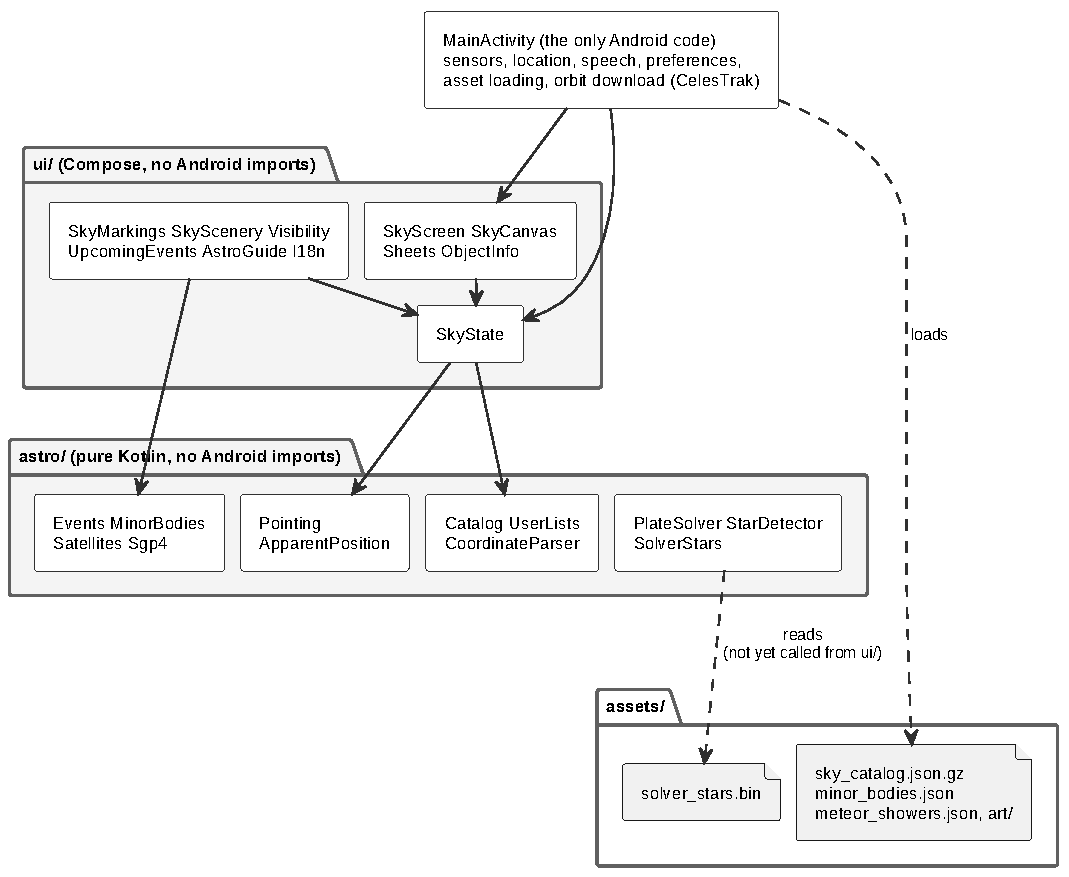
\includegraphics[width=0.8\textwidth]{figures/uml02_components.pdf}
\caption{Components of the app and the assets they read. Dashed arrows are data access}
\label{fig:components}
\end{figure*}

Figure~\ref{fig:classes}(a) gives the core classes. \texttt{SkyState} holds what the screen shows: time, place, phone rotation, pointing mode, alignment state and matrix, the target and the eyepiece settings. Its guidance methods combine the camera frame from \texttt{Pointing} with the ray to the target. \texttt{Catalog} owns the \texttt{SkyObject} list and answers cone, name and constellation queries. The members below the dotted line in \texttt{SkyState}, and \texttt{TelescopeSetup} with its enumerations, exist only in the development branch.


Figure~\ref{fig:classes}(b) shows the solver classes. \texttt{PlateSolver} has two entry points, \texttt{detectStars} and \texttt{solve}. The \texttt{StarSource} interface lets the same solver run on the bright catalogue through \texttt{CatalogStars}, on the 580k-star file through \texttt{SolverStars}, or on a plain list in tests. The result is a sealed class: \texttt{Solved} carries the pose and the false-alarm probability, and \texttt{Failed} carries one of four reasons.

\begin{figure*}[tp]
\centering
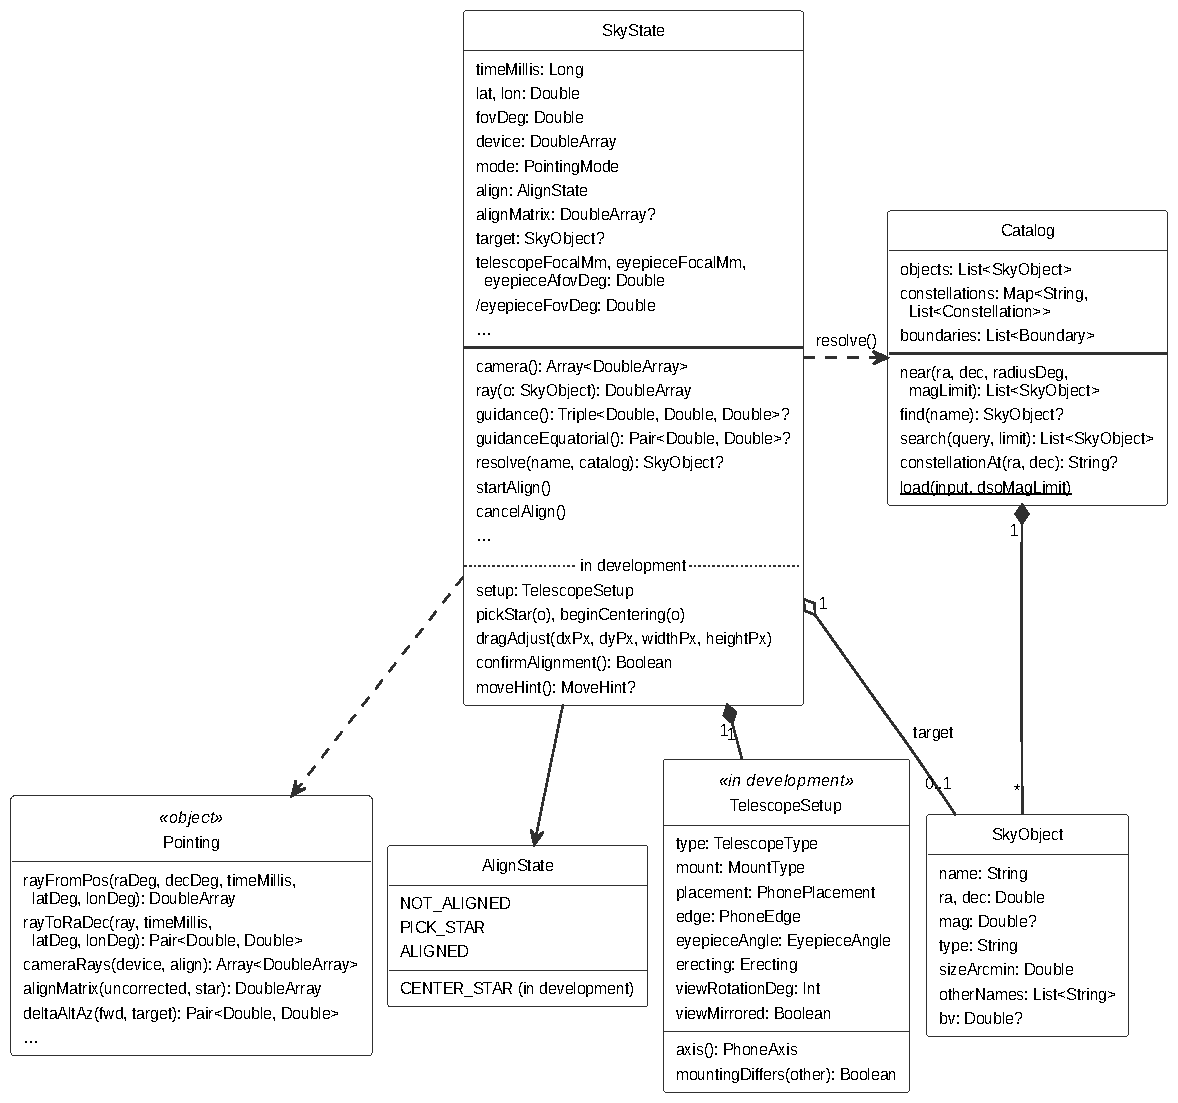
\includegraphics[width=0.72\textwidth]{figures/uml03a_classes_core.pdf}\\[2pt]
(a)\\[6pt]
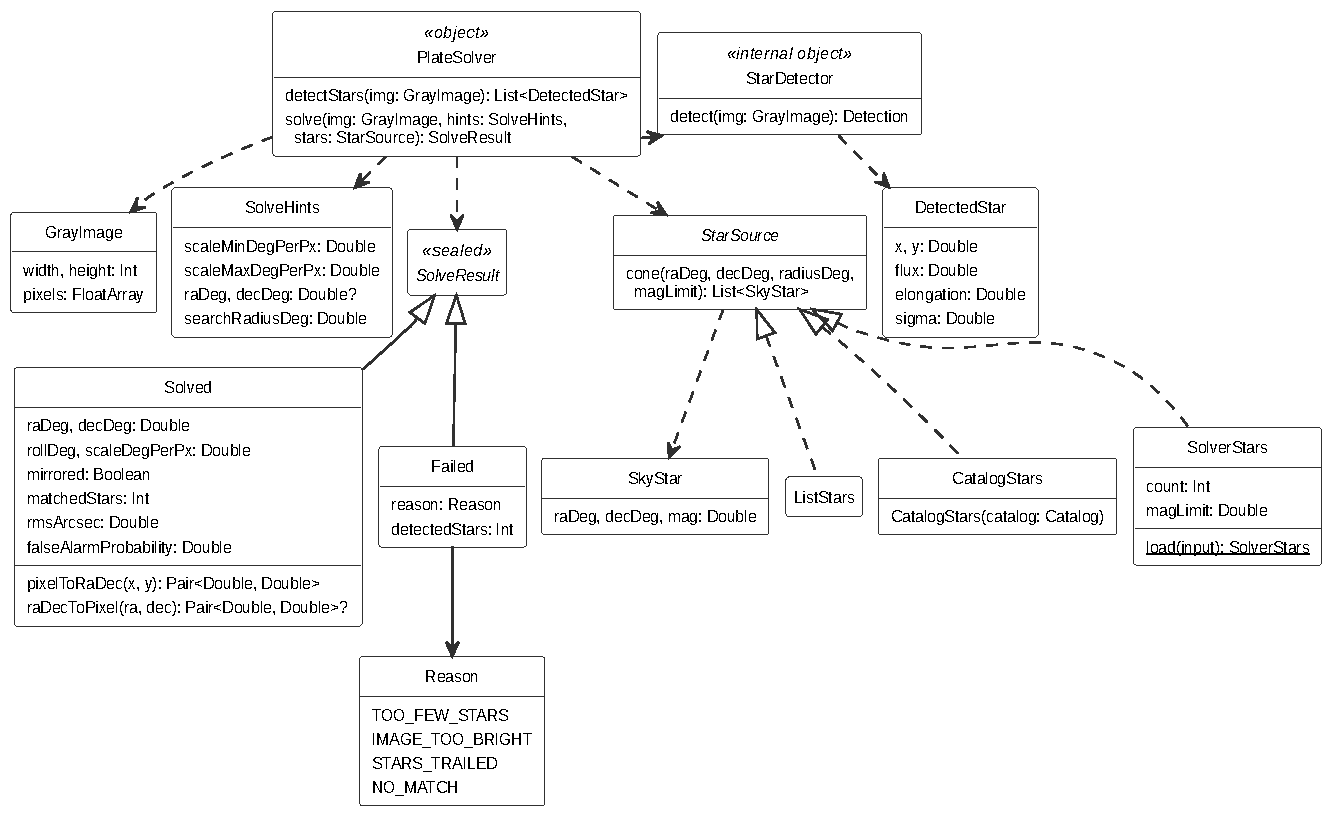
\includegraphics[width=0.76\textwidth]{figures/uml03b_classes_solver.pdf}\\[2pt]
(b)
\caption{Classes of (a) the core model and (b) the plate solver. Members marked in development are not in the released build}
\label{fig:classes}
\end{figure*}

\subsection{Alignment and plate solving}

Figure~\ref{fig:states} shows the alignment states of the revised flow. In the current build, tapping a star while picking aligns at once, as if the telescope were already centred. The revised flow inserts a centring state, so nothing is calibrated until the observer confirms. Cancelling returns to the aligned state if a calibration exists and to the unaligned state otherwise. The calibration is cleared when the phone mounting changes or the settings are reset.

\begin{figure*}[tp]
\centering
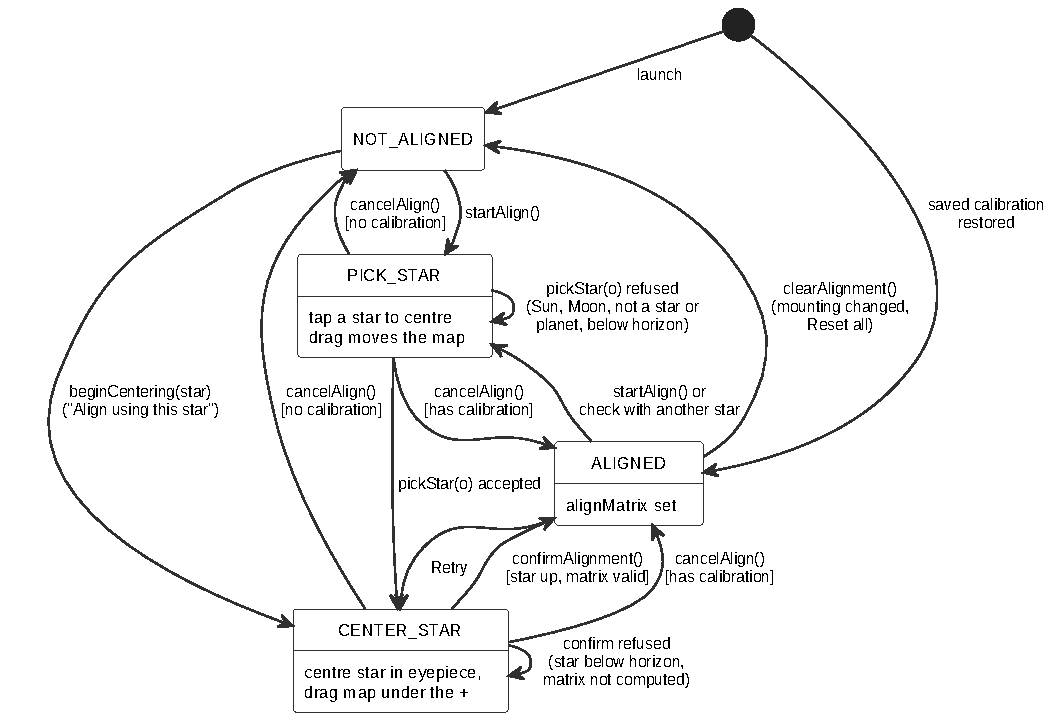
\includegraphics[width=0.7\textwidth]{figures/uml04_states.pdf}
\caption{Alignment states and transitions, from \texttt{SkyState} (in development)}
\label{fig:states}
\end{figure*}

Figure~\ref{fig:sequence} follows one alignment through the classes. The observer starts alignment and taps a star. \texttt{SkyState} accepts it unless it is the Sun, the Moon, not a star or planet, or below the horizon. Dragging the map only changes a pending adjustment, so browsing cannot change the calibration. Confirming computes \texttt{alignMatrix} from the uncorrected camera frame and the star, and rejects it if the corrected axis does not land on the star.

\begin{figure}[tbp]
\centering
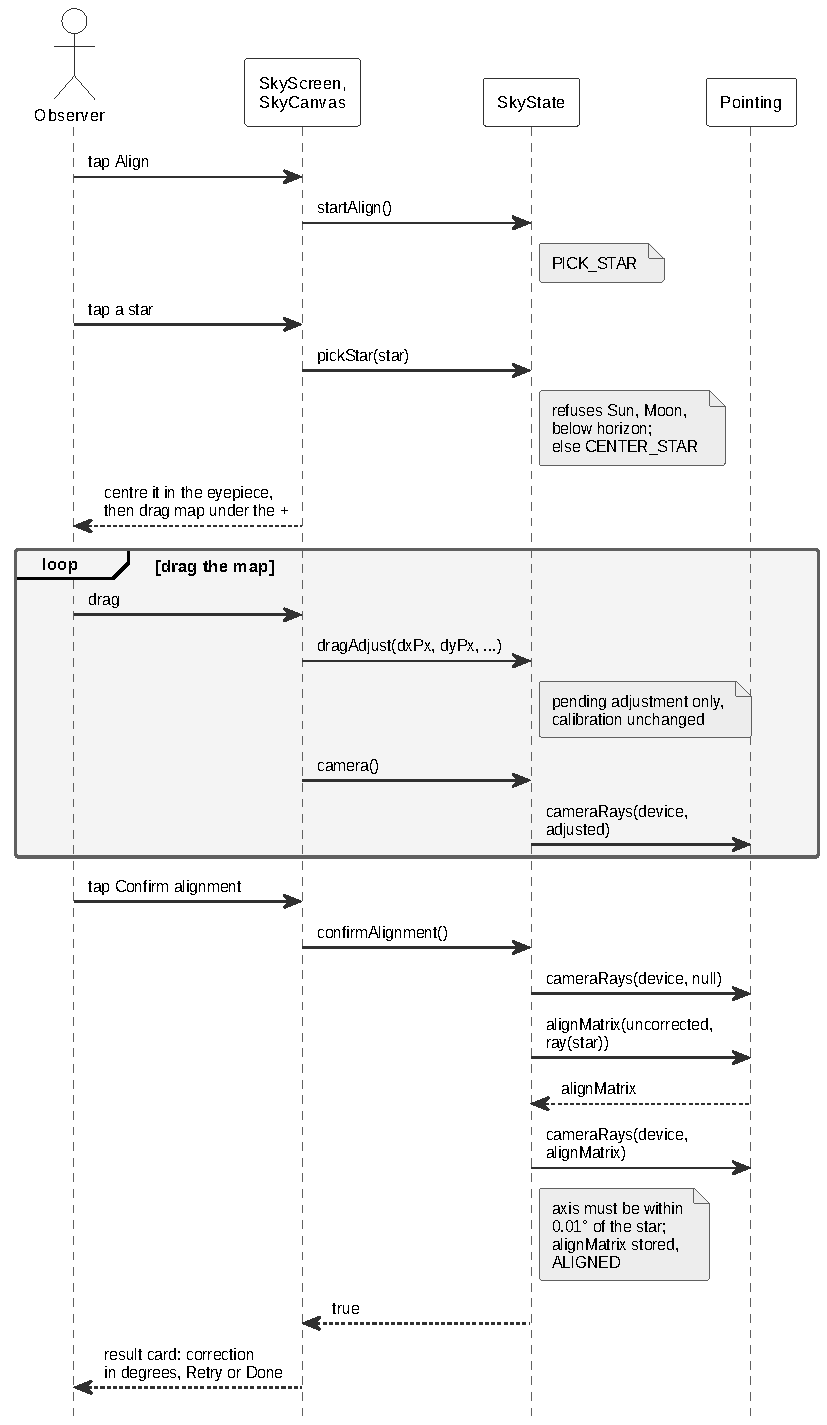
\includegraphics[width=0.9\columnwidth]{figures/uml05_sequence.pdf}
\caption{Star alignment with drag to align (in development)}
\label{fig:sequence}
\end{figure}

Figure~\ref{fig:activity} shows the plate solve as an activity. The three early checks reject a bad image before any matching starts and tell the observer which problem was found. Matching then builds hypotheses from triangles, and each hypothesis is verified against the catalogue. A result is accepted only if it passes the acceptance test described in Section~\ref{sec:solver}; otherwise the solver reports no match.

\begin{figure}[tbp]
\centering
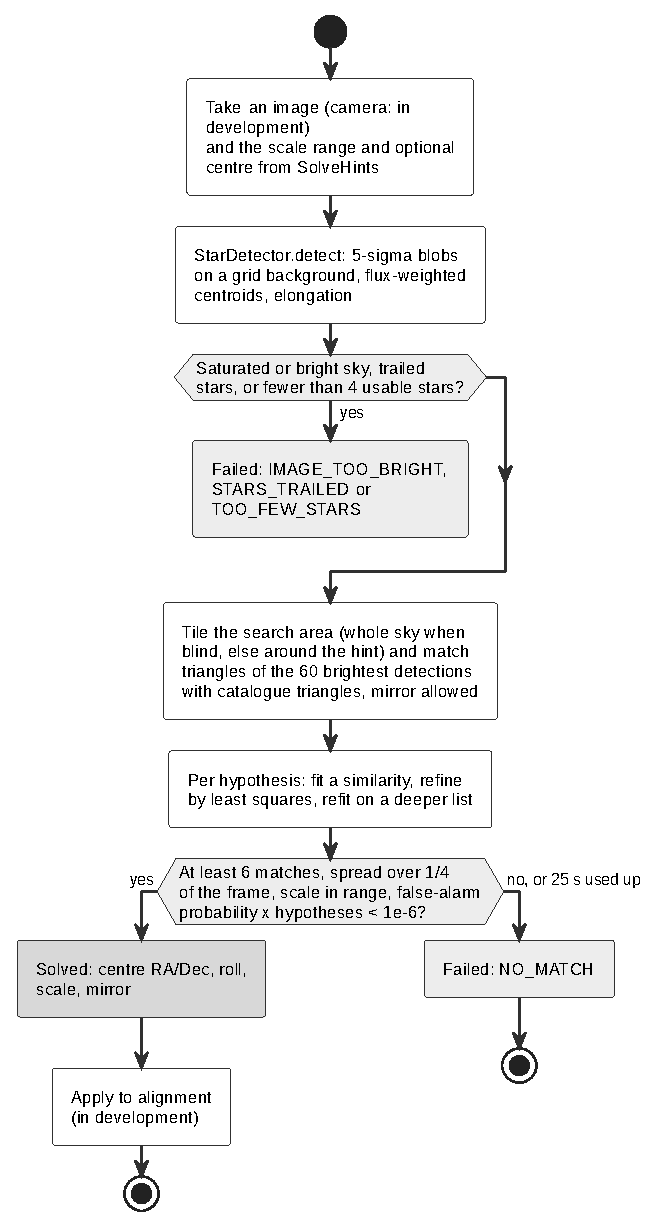
\includegraphics[width=0.8\columnwidth]{figures/uml06_activity.pdf}
\caption{Plate solve, from \texttt{PlateSolver} and \texttt{StarDetector}. Camera capture and applying the result to the alignment are in development}
\label{fig:activity}
\end{figure}

\subsection{Build, test and release}

Figure~\ref{fig:deployment} shows how the code becomes an installed app. The developer runs the importer to write the data assets and pushes the source. Three GitHub Actions jobs run on every push: \texttt{build} runs the JVM tests, assembles the APKs and checks that the sky data is inside the package; \texttt{ui-check} runs the desktop tests and saves screenshots; and \texttt{secret-scan} runs gitleaks over the whole history. A push to the main branch also publishes the latest APK as a GitHub release, and a version tag starts a separate workflow that builds a signed bundle and APK. The phone downloads the APK and needs no network afterwards, except to refresh satellite orbits.

\begin{figure*}[tp]
\centering
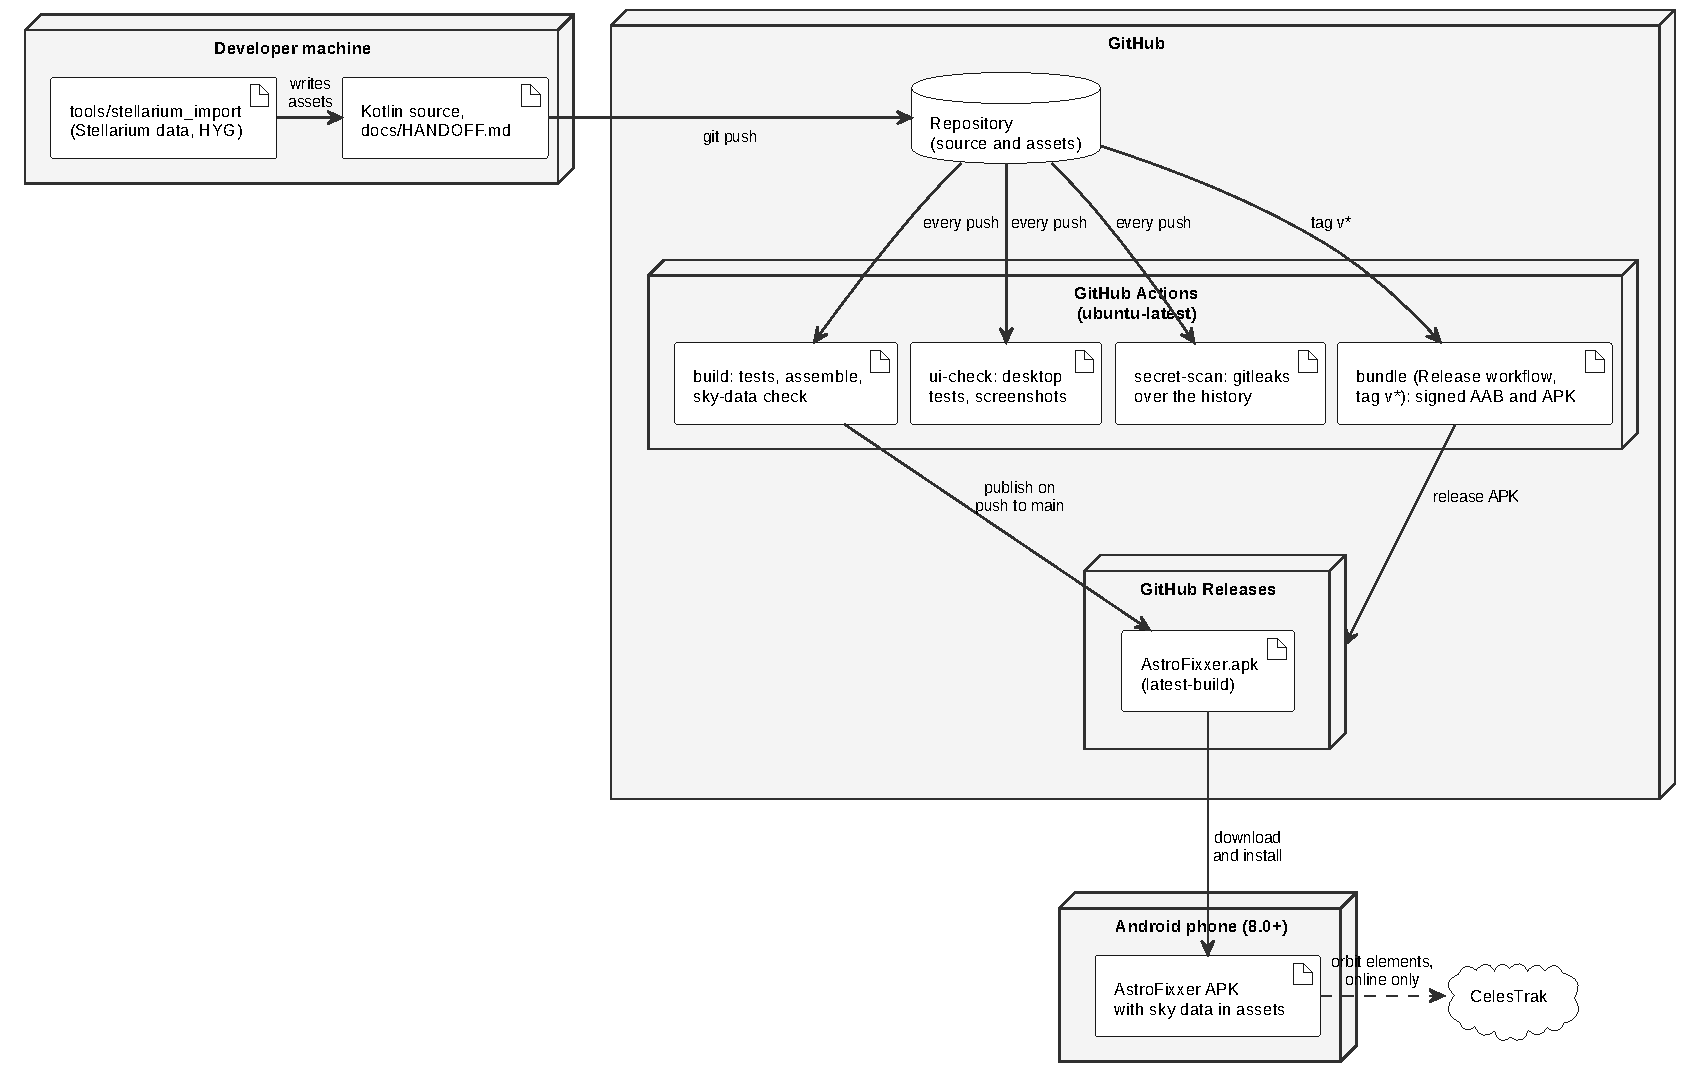
\includegraphics[width=\textwidth]{figures/uml07_deployment.pdf}
\caption{Deployment: from the developer machine through GitHub Actions to the phone}
\label{fig:deployment}
\end{figure*}

\subsection{Development process}

Figure~\ref{fig:process} lists the phases the project followed. Work started from an analysis of the web application and a plan, and the plan went through a review that climbs a ladder of questions (does it need to exist, is it already in the code, does the platform provide it) before any code is written. Each change ends with tests, an entry in the handoff log and a push that starts the CI jobs above. The current phase, 7b, adds the precession fix, the plate solver and the setup and alignment work; the last of these is still open, and the field test is written but has not been run.

\begin{figure}[tbp]
\centering
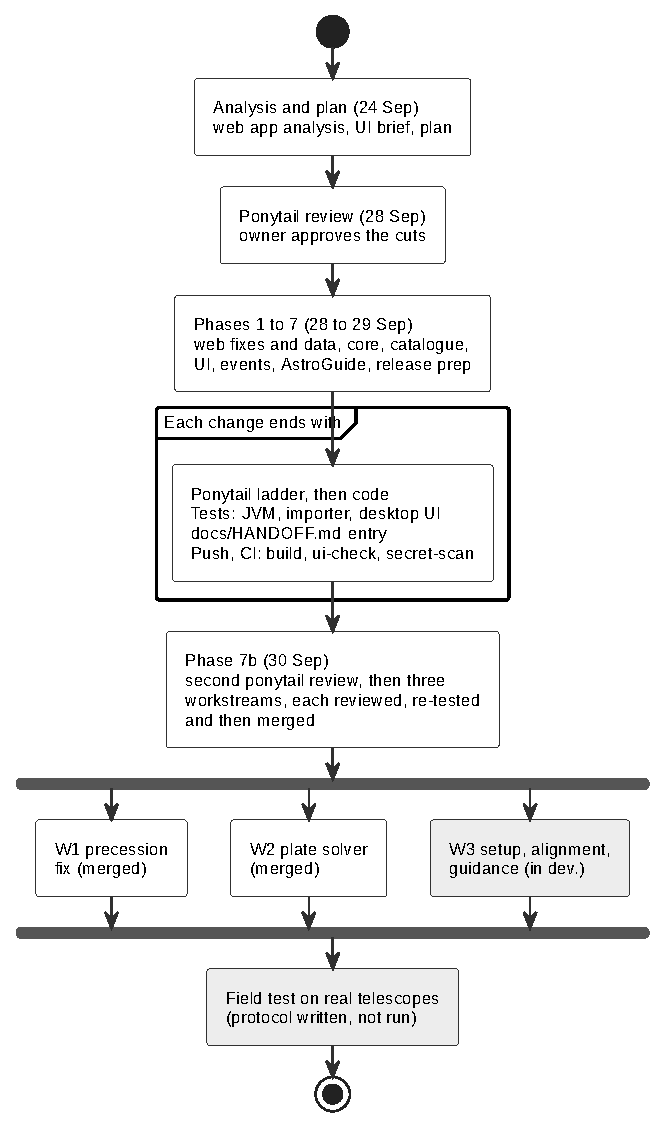
\includegraphics[width=0.75\columnwidth]{figures/uml08_process.pdf}
\caption{Development phases and the steps that end each change}
\label{fig:process}
\end{figure}
